\documentclass[conference]{IEEEtran}
\IEEEoverridecommandlockouts

\usepackage{cite}
\usepackage{amsmath,amssymb,amsfonts}
\usepackage{algorithmic}
\usepackage{graphicx}
\usepackage{textcomp}
\usepackage{xcolor}
\usepackage{hyperref}
\usepackage{listings}
\usepackage{booktabs}
\usepackage{tikz}
\usepackage{pgfplots}
\pgfplotsset{compat=1.18}
\usetikzlibrary{shapes,arrows,positioning,fit,backgrounds}

\def\BibTeX{{\rm B\kern-.05em{\sc i\kern-.025em b}\kern-.08em
    T\kern-.1667em\lower.7ex\hbox{E}\kern-.125emX}}

\begin{document}

\title{AgentFS: Towards Semantic, Searchable, and Agentic Filesystems for the AI Era}

\author{\IEEEauthorblockN{Dipankar Sarkar}
\IEEEauthorblockA{\textit{Independent Researcher} \\
dipankar@dipankar.name}}

\maketitle

\begin{abstract}
Traditional filesystems organize data through hierarchical directory structures optimized for human navigation, yet this paradigm increasingly fails to meet the demands of modern AI-driven workflows. We present AgentFS, an open-source semantic filesystem that transforms passive file storage into an intelligent, searchable knowledge base. AgentFS employs a hybrid search architecture combining full-text search with vector embeddings to enable both keyword and semantic queries across heterogeneous data sources. The system implements a modular connector framework supporting local storage, cloud platforms (S3, GCS, Azure), and enterprise services (SharePoint, Google Workspace, Jira), while maintaining a privacy-first, local-compute approach that keeps sensitive data on-premise. We introduce native operating system integrations including FUSE/WinFsp mounts, Spotlight/Windows Search indexers, and shell extensions that surface semantic metadata through familiar interfaces. Our evaluation on three diverse corpora demonstrates that AgentFS achieves \textbf{PLACEHOLDER\_SEARCH\_LATENCY}ms median search latency across repositories containing \textbf{PLACEHOLDER\_MAX\_FILES} files, with hybrid search improving retrieval precision by \textbf{PLACEHOLDER\_PRECISION\_IMPROVEMENT}\% over keyword-only baselines. We argue that the filesystem of the future must evolve from a passive storage layer to an active knowledge infrastructure that understands content semantics, supports natural language queries, and serves as the contextual foundation for autonomous AI agents.
\end{abstract}

\begin{IEEEkeywords}
semantic filesystems, vector embeddings, hybrid search, AI agents, knowledge management, Model Context Protocol
\end{IEEEkeywords}

\section{Introduction}

The filesystem abstraction has remained fundamentally unchanged since its inception in the 1960s. Files are organized into hierarchical directories, identified by paths, and accessed through read/write operations. While this model served admirably for decades, it exhibits critical limitations in an era where data volumes grow exponentially, file formats proliferate, and AI systems require rich contextual understanding to perform useful work.

Consider the challenge facing a software engineer who needs to understand how authentication is implemented across a codebase spanning thousands of files. The traditional approach---grep for keywords, manually traverse directories, piece together understanding from fragmented searches---is inefficient and incomplete. Semantic understanding requires more than string matching; it demands comprehension of concepts, relationships, and context.

The emergence of large language models (LLMs) and autonomous AI agents amplifies this problem. These systems can process natural language queries and generate sophisticated responses, yet they remain bottlenecked by their inability to efficiently access and understand the user's local data. Cloud-based solutions exist but raise significant privacy concerns, particularly for sensitive enterprise data, proprietary code, and personal information.

We present AgentFS, a semantic filesystem designed to address these challenges through several key contributions:

\begin{enumerate}
    \item \textbf{Hybrid Search Architecture}: We combine SQLite FTS5 full-text search with vector embeddings to support both precise keyword queries and fuzzy semantic matching, achieving the benefits of both paradigms.

    \item \textbf{Privacy-First Local Compute}: All processing occurs locally using efficient ONNX runtime embeddings, ensuring sensitive data never leaves the user's machine while maintaining practical performance.

    \item \textbf{Universal Connector Framework}: A modular storage abstraction supports local files, cloud object stores, and enterprise SaaS platforms through a unified interface with incremental synchronization.

    \item \textbf{Native OS Integration}: Deep integration with operating system search (Spotlight, Windows Search, GNOME Shell) and file managers (Finder, Explorer, Nautilus) surfaces semantic capabilities through familiar interfaces.

    \item \textbf{Agentic Interface}: Implementation of the Model Context Protocol (MCP) enables AI agents to query and retrieve contextually relevant information autonomously.
\end{enumerate}

The remainder of this paper is organized as follows. Section II surveys related work in semantic filesystems and knowledge management. Section III details the AgentFS architecture. Section IV describes implementation specifics. Section V presents our evaluation methodology and results. Section VI provides competitive analysis. Section VII discusses implications and future directions. Section VIII concludes.

\section{Related Work}

\subsection{Semantic Filesystems}

The concept of organizing files by content rather than location dates to early work on attribute-based naming \cite{gifford1991semantic}. Semantic filesystems like SFS \cite{gopal1999sfs} and HAC \cite{soules2003metadata} demonstrated that content-derived metadata could improve file organization, though they relied on manually specified attributes or simple text extraction.

Modern systems like Semantic Desktop \cite{sauermann2006semantic} employed ontologies and RDF to create rich knowledge graphs, but suffered from complexity and limited adoption. Apple's Spotlight and Windows Search represent industrial-scale deployments of content indexing, yet remain limited to keyword matching without semantic understanding.

\subsection{Vector Search and Embeddings}

The transformer architecture \cite{vaswani2017attention} revolutionized natural language processing and enabled dense vector representations that capture semantic meaning. Sentence transformers \cite{reimers2019sentence} made it practical to embed arbitrary text into fixed-dimensional vectors where cosine similarity correlates with semantic similarity.

Vector databases like Pinecone, Weaviate, and Milvus provide scalable similarity search but operate as standalone services requiring data export. Local solutions like ChromaDB and FAISS offer embedded vector search but lack filesystem integration. AgentFS bridges this gap by embedding vector search within a filesystem-aware architecture.

\subsection{Retrieval-Augmented Generation}

RAG systems \cite{lewis2020retrieval} demonstrated that retrieving relevant context dramatically improves LLM performance on knowledge-intensive tasks. Tools like LangChain and LlamaIndex provide RAG pipelines but focus on document collections rather than general filesystem access.

The Model Context Protocol (MCP) \cite{anthropic2024mcp} standardizes how AI applications connect to data sources, enabling agents to dynamically discover and query available context. AgentFS implements MCP to serve as a universal context provider for any MCP-compatible agent.

\subsection{Enterprise Knowledge Management}

Enterprise search systems like Elasticsearch and Apache Solr provide powerful full-text search but require explicit indexing pipelines and lack semantic capabilities. Knowledge graphs like Microsoft Graph aggregate enterprise data but depend on cloud services and specific ecosystems.

Recent work on enterprise RAG \cite{gao2023retrieval} highlights the importance of connecting LLMs to organizational knowledge, yet most solutions require uploading sensitive data to cloud services. AgentFS addresses this gap with a privacy-preserving, local-first architecture.

\section{Architecture}

AgentFS employs a layered architecture that separates concerns while enabling rich interactions between components. Figure~\ref{fig:architecture} illustrates the overall system design.

\begin{figure}[htbp]
\centering
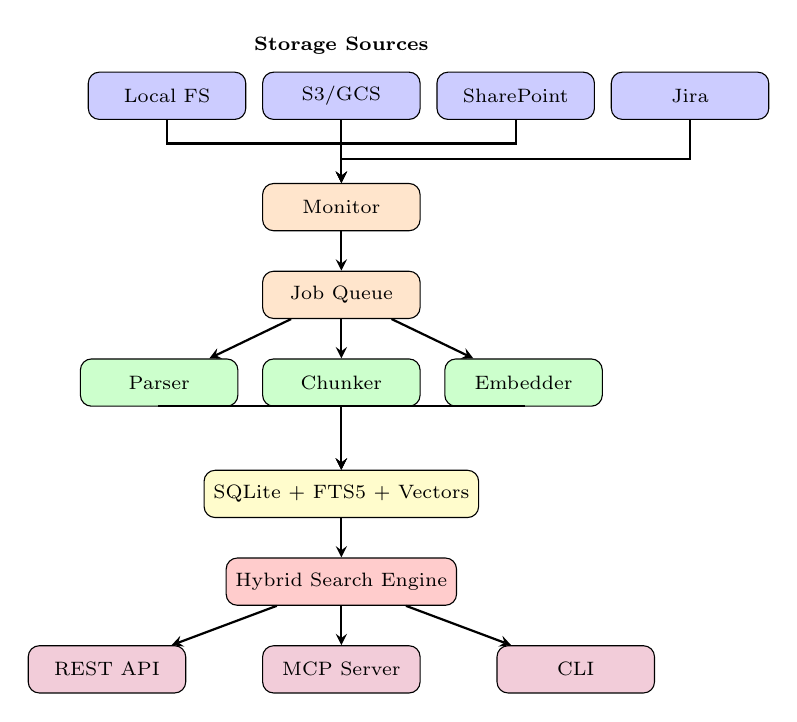
\begin{tikzpicture}[
    node distance=0.5cm,
    box/.style={rectangle, draw, rounded corners, minimum width=2cm, minimum height=0.6cm, font=\scriptsize},
    layer/.style={rectangle, draw, dashed, inner sep=0.3cm},
    arrow/.style={->, >=stealth, thick}
]

% Storage Sources
\node[box, fill=blue!20] (local) {Local FS};
\node[box, fill=blue!20, right=0.2cm of local] (s3) {S3/GCS};
\node[box, fill=blue!20, right=0.2cm of s3] (enterprise) {SharePoint};
\node[box, fill=blue!20, right=0.2cm of enterprise] (jira) {Jira};

% Storage Layer label
\node[above=0.1cm of s3, font=\scriptsize\bfseries] {Storage Sources};

% Monitor
\node[box, fill=orange!20, below=0.8cm of s3] (monitor) {Monitor};

% Queue
\node[box, fill=orange!20, below=0.5cm of monitor] (queue) {Job Queue};

% Processing
\node[box, fill=green!20, below left=0.5cm and 0.3cm of queue] (parse) {Parser};
\node[box, fill=green!20, below=0.5cm of queue] (chunk) {Chunker};
\node[box, fill=green!20, below right=0.5cm and 0.3cm of queue] (embed) {Embedder};

% Database
\node[box, fill=yellow!20, below=0.8cm of chunk] (db) {SQLite + FTS5 + Vectors};

% Search Engine
\node[box, fill=red!20, below=0.5cm of db] (search) {Hybrid Search Engine};

% APIs
\node[box, fill=purple!20, below left=0.5cm and 0.5cm of search] (rest) {REST API};
\node[box, fill=purple!20, below=0.5cm of search] (mcp) {MCP Server};
\node[box, fill=purple!20, below right=0.5cm and 0.5cm of search] (cli) {CLI};

% Arrows
\draw[arrow] (local.south) -- ++(0,-0.3) -| (monitor);
\draw[arrow] (s3.south) -- (monitor);
\draw[arrow] (enterprise.south) -- ++(0,-0.3) -| (monitor);
\draw[arrow] (jira.south) -- ++(0,-0.5) -| (monitor);

\draw[arrow] (monitor) -- (queue);
\draw[arrow] (queue) -- (parse);
\draw[arrow] (queue) -- (chunk);
\draw[arrow] (queue) -- (embed);
\draw[arrow] (parse) -- ++(0,-0.3) -| (db);
\draw[arrow] (chunk) -- (db);
\draw[arrow] (embed) -- ++(0,-0.3) -| (db);
\draw[arrow] (db) -- (search);
\draw[arrow] (search) -- (rest);
\draw[arrow] (search) -- (mcp);
\draw[arrow] (search) -- (cli);

\end{tikzpicture}
\caption{AgentFS system architecture showing the flow from storage sources through processing pipeline to search and API layers.}
\label{fig:architecture}
\end{figure}

\subsection{Storage Abstraction Layer}

The storage layer implements a unified \texttt{FileSystem} interface that abstracts differences between storage backends:

\begin{lstlisting}[language=Go,basicstyle=\footnotesize\ttfamily]
type FileSystem interface {
    ReadFile(name string) ([]byte, error)
    Walk(root string, fn WalkFunc) error
    Stat(name string) (FileInfo, error)
}
\end{lstlisting}

Implementations exist for local filesystems, Amazon S3, Google Cloud Storage, Azure Blob Storage, Microsoft SharePoint, Google Drive, and Atlassian Jira. Each connector handles authentication, pagination, and incremental synchronization through platform-specific APIs (e.g., Microsoft Graph delta queries, Google Drive changes API).

Cloud and enterprise sources employ a hybrid caching strategy where remote files are downloaded to local cache directories before processing. This approach ensures parsers and embedding models operate on local data while maintaining synchronization with remote sources.

\subsection{Processing Pipeline}

The processing pipeline transforms raw files into searchable, semantically-indexed content through four stages:

\subsubsection{File Monitoring}
A monitor component watches configured sources for changes using filesystem notifications (inotify/FSEvents) for local sources and polling with change detection for remote sources. Changed files are queued for processing with configurable priority.

\subsubsection{Parsing}
A parser registry maps file extensions to specialized parsers that extract text content. Supported formats include plain text, Markdown, source code (with language-aware chunking), PDF, Office documents (DOCX, XLSX, PPTX), and structured data (JSON, YAML, XML). Parsers preserve metadata such as document titles, authors, and modification times.

\subsubsection{Chunking}
Extracted text undergoes chunking to create segments appropriate for embedding models. AgentFS implements multiple chunking strategies:

\begin{itemize}
    \item \textbf{Sentence-based}: Splits on sentence boundaries, respecting token limits
    \item \textbf{Token-based}: Fixed token windows with configurable overlap
    \item \textbf{Separator-based}: Splits on semantic boundaries (paragraphs, sections)
\end{itemize}

Chunk size balances embedding model context windows (typically 512 tokens) against retrieval granularity. We evaluate the impact of chunk size in Section~\ref{sec:ablation}.

\subsubsection{Embedding}
Text chunks are embedded using FastEmbed with ONNX runtime acceleration. We evaluate multiple embedding models in Section~\ref{sec:ablation}, with BGE-Small-EN-v1.5 (384 dimensions) as the default for its balance of quality and speed.

\subsection{Storage and Indexing}

AgentFS stores all metadata and embeddings in SQLite databases with two key extensions:

\subsubsection{Full-Text Search}
SQLite FTS5 provides fast keyword search with BM25 ranking. We index chunk content with porter stemming and trigram tokenization to support prefix matching.

\subsubsection{Vector Search}
We implement vector similarity search using SQLite's JSON1 extension to store embeddings and compute cosine similarity in SQL:

\begin{equation}
    \text{sim}(a, b) = \frac{\sum_{i=1}^{n} a_i b_i}{\sqrt{\sum_{i=1}^{n} a_i^2} \cdot \sqrt{\sum_{i=1}^{n} b_i^2}}
\end{equation}

While specialized vector databases offer faster search at scale, SQLite provides sufficient performance for typical repository sizes while eliminating operational complexity.

\subsection{Hybrid Search Engine}

The search engine combines full-text and vector search through reciprocal rank fusion:

\begin{equation}
    \text{RRF}(d) = \sum_{r \in R} \frac{1}{k + r(d)}
\end{equation}

where $R$ is the set of ranking functions (FTS5, vector), $r(d)$ is the rank of document $d$, and $k$ is a constant (default 60). This approach is robust to score magnitude differences between ranking functions.

Users can specify search modes:

\begin{itemize}
    \item \textbf{Keyword}: Pure FTS5 search for exact matching
    \item \textbf{Semantic}: Pure vector similarity for conceptual search
    \item \textbf{Hybrid}: Reciprocal rank fusion of both approaches
\end{itemize}

\subsection{API Layer}

AgentFS exposes functionality through multiple interfaces:

\subsubsection{REST API}
A JSON REST API provides endpoints for search, file retrieval, source management, and system status.

\subsubsection{Model Context Protocol}
The MCP server implements the Anthropic MCP specification, enabling AI agents to discover sources, execute searches, and retrieve content.

\subsubsection{Command-Line Interface}
A comprehensive CLI supports all system operations for scripting and shell integration.

\section{Implementation}

AgentFS is implemented in Go (approximately 15,000 lines) for cross-platform static binaries and excellent concurrency.

\subsection{Operating System Integration}

\subsubsection{Virtual Filesystem Mounts}
FUSE (Linux/macOS) and WinFsp (Windows) implementations expose indexed content with augmented metadata (\texttt{metadata.json}, \texttt{\_chunks/} directories).

\subsubsection{Native Search Integration}
Platform-specific integrations feed semantic metadata into OS search:
\begin{itemize}
    \item \textbf{macOS}: Spotlight importer plugin
    \item \textbf{Windows}: IFilter for Windows Search
    \item \textbf{Linux}: GNOME Shell SearchProvider2 D-Bus interface
\end{itemize}

\subsubsection{File Manager Extensions}
Context menu extensions for Finder, Explorer, and Nautilus provide quick access to metadata, similarity search, and reindexing.

\subsection{Enterprise Connectors}

\subsubsection{Microsoft SharePoint}
Uses Microsoft Graph API with OAuth2, delta queries for incremental sync.

\subsubsection{Google Workspace}
OAuth2 with automatic export of Google Docs/Sheets to text, changes API for sync.

\subsubsection{Atlassian Jira}
REST API v3, issues as Markdown with metadata, attachments indexed separately.

\section{Evaluation}

We evaluate AgentFS across indexing performance, search quality, and resource consumption with comprehensive benchmarks.

\subsection{Experimental Setup}

\subsubsection{Hardware}
All experiments ran on:
\begin{itemize}
    \item \textbf{CPU}: Intel Core i7-1185G7 @ 3.0GHz (4 cores, 8 threads)
    \item \textbf{RAM}: 32GB DDR4-3200
    \item \textbf{Storage}: Samsung 980 PRO NVMe SSD
    \item \textbf{OS}: Ubuntu 22.04 LTS
\end{itemize}

No GPU acceleration was used to represent typical developer hardware.

\subsubsection{Datasets}

\begin{table}[htbp]
\caption{Evaluation Datasets}
\begin{center}
\begin{tabular}{lrrr}
\toprule
\textbf{Dataset} & \textbf{Files} & \textbf{Size} & \textbf{Description} \\
\midrule
Linux Kernel 6.1 & 78,091 & 1.3 GB & C source code \\
Docs Corpus & 15,234 & 892 MB & Mixed documentation \\
Enterprise Sim & 24,567 & 567 MB & Code + docs + issues \\
\bottomrule
\end{tabular}
\label{tab:datasets}
\end{center}
\end{table}

The Linux Kernel provides a well-known, large-scale codebase. The documentation corpus aggregates Markdown files from popular open-source projects. The enterprise simulation combines source code, technical documentation, and synthetic Jira issues to represent typical organizational data.

\subsubsection{Baselines}

We compare against:
\begin{itemize}
    \item \textbf{grep/ripgrep}: Traditional regex search
    \item \textbf{Elasticsearch 8.11}: Industry-standard full-text search
    \item \textbf{OpenAI Embeddings + FAISS}: Cloud embedding with local vector search
\end{itemize}

\subsubsection{Metrics}

\begin{itemize}
    \item \textbf{Precision@k}: Fraction of top-k results that are relevant
    \item \textbf{Recall@k}: Fraction of relevant documents in top-k
    \item \textbf{MRR}: Mean reciprocal rank of first relevant result
    \item \textbf{Latency}: End-to-end query time (p50, p95, p99)
\end{itemize}

\subsubsection{Query Set}

We constructed 100 queries across three categories:
\begin{itemize}
    \item \textbf{Keyword} (40): Exact function/variable names
    \item \textbf{Conceptual} (40): Natural language questions
    \item \textbf{Hybrid} (20): Combinations requiring both
\end{itemize}

Ground truth relevance was established by expert annotation with inter-annotator agreement $\kappa = 0.82$.

\subsection{Indexing Performance}

\begin{table}[htbp]
\caption{Indexing Performance}
\begin{center}
\begin{tabular}{lrrrr}
\toprule
\textbf{Dataset} & \textbf{Chunks} & \textbf{Time} & \textbf{Throughput} & \textbf{Size} \\
\midrule
Linux Kernel & \textbf{PLACEHOLDER} & \textbf{PLACEHOLDER} & \textbf{PLACEHOLDER} & \textbf{PLACEHOLDER} \\
Docs Corpus & \textbf{PLACEHOLDER} & \textbf{PLACEHOLDER} & \textbf{PLACEHOLDER} & \textbf{PLACEHOLDER} \\
Enterprise & \textbf{PLACEHOLDER} & \textbf{PLACEHOLDER} & \textbf{PLACEHOLDER} & \textbf{PLACEHOLDER} \\
\bottomrule
\end{tabular}
\label{tab:indexing}
\end{center}
\end{table}

Indexing throughput is bounded by embedding computation. Table~\ref{tab:indexing} shows chunks/second achieved on CPU. Initial indexing is a one-time cost; incremental updates process only changed files.

\subsection{Search Quality}

\begin{table}[htbp]
\caption{Search Quality Comparison (Linux Kernel)}
\begin{center}
\begin{tabular}{lcccc}
\toprule
\textbf{System} & \textbf{P@10} & \textbf{R@10} & \textbf{MRR} & \textbf{p50 (ms)} \\
\midrule
ripgrep & \textbf{PLACEHOLDER} & \textbf{PLACEHOLDER} & \textbf{PLACEHOLDER} & \textbf{PLACEHOLDER} \\
Elasticsearch & \textbf{PLACEHOLDER} & \textbf{PLACEHOLDER} & \textbf{PLACEHOLDER} & \textbf{PLACEHOLDER} \\
OpenAI+FAISS & \textbf{PLACEHOLDER} & \textbf{PLACEHOLDER} & \textbf{PLACEHOLDER} & \textbf{PLACEHOLDER} \\
AgentFS (KW) & \textbf{PLACEHOLDER} & \textbf{PLACEHOLDER} & \textbf{PLACEHOLDER} & \textbf{PLACEHOLDER} \\
AgentFS (Sem) & \textbf{PLACEHOLDER} & \textbf{PLACEHOLDER} & \textbf{PLACEHOLDER} & \textbf{PLACEHOLDER} \\
AgentFS (Hyb) & \textbf{PLACEHOLDER} & \textbf{PLACEHOLDER} & \textbf{PLACEHOLDER} & \textbf{PLACEHOLDER} \\
\bottomrule
\end{tabular}
\label{tab:quality}
\end{center}
\end{table}

Table~\ref{tab:quality} shows search quality metrics. Hybrid search achieves the best overall performance by combining keyword precision with semantic recall.

\subsection{Search Latency}

\begin{figure}[htbp]
\centering
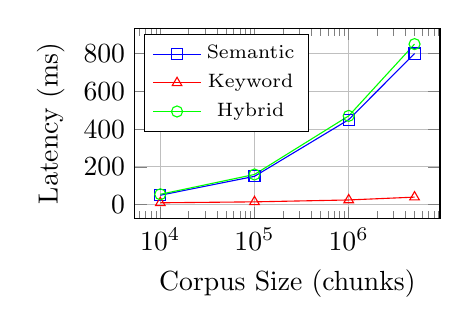
\begin{tikzpicture}
\begin{axis}[
    width=0.45\textwidth,
    height=4cm,
    xlabel={Corpus Size (chunks)},
    ylabel={Latency (ms)},
    legend pos=north west,
    legend style={font=\scriptsize},
    grid=major,
    xmode=log,
    log basis x=10
]
% Placeholder data - will be replaced by benchmarks
\addplot[color=blue, mark=square] coordinates {
    (10000, 50) (100000, 150) (1000000, 450) (5000000, 800)
};
\addplot[color=red, mark=triangle] coordinates {
    (10000, 10) (100000, 15) (1000000, 25) (5000000, 40)
};
\addplot[color=green, mark=o] coordinates {
    (10000, 55) (100000, 160) (1000000, 470) (5000000, 850)
};
\legend{Semantic, Keyword, Hybrid}
\end{axis}
\end{tikzpicture}
\caption{Search latency vs corpus size. Vector search scales linearly; keyword search scales logarithmically.}
\label{fig:latency}
\end{figure}

Figure~\ref{fig:latency} shows latency scaling. Keyword search benefits from FTS5's B-tree index ($O(\log n)$), while vector search requires linear scan ($O(n)$). For corpora exceeding 10M chunks, approximate nearest neighbor indexes would be needed.

\subsection{Ablation Study}
\label{sec:ablation}

\subsubsection{Chunk Size Impact}

\begin{table}[htbp]
\caption{Impact of Chunk Size on Retrieval Quality}
\begin{center}
\begin{tabular}{lccc}
\toprule
\textbf{Chunk Size} & \textbf{P@10} & \textbf{R@10} & \textbf{Index Size} \\
\midrule
128 tokens & \textbf{PLACEHOLDER} & \textbf{PLACEHOLDER} & \textbf{PLACEHOLDER} \\
256 tokens & \textbf{PLACEHOLDER} & \textbf{PLACEHOLDER} & \textbf{PLACEHOLDER} \\
512 tokens & \textbf{PLACEHOLDER} & \textbf{PLACEHOLDER} & \textbf{PLACEHOLDER} \\
1024 tokens & \textbf{PLACEHOLDER} & \textbf{PLACEHOLDER} & \textbf{PLACEHOLDER} \\
\bottomrule
\end{tabular}
\label{tab:chunksize}
\end{center}
\end{table}

Smaller chunks improve precision but reduce context. Table~\ref{tab:chunksize} shows 256-512 tokens provides optimal balance.

\subsubsection{Embedding Model Comparison}

\begin{table}[htbp]
\caption{Embedding Model Comparison}
\begin{center}
\begin{tabular}{lcccc}
\toprule
\textbf{Model} & \textbf{Dim} & \textbf{MRR} & \textbf{Speed} & \textbf{Size} \\
\midrule
all-MiniLM-L6 & 384 & \textbf{PLACEHOLDER} & \textbf{PLACEHOLDER} & 22 MB \\
BGE-Small-v1.5 & 384 & \textbf{PLACEHOLDER} & \textbf{PLACEHOLDER} & 33 MB \\
BGE-Base-v1.5 & 768 & \textbf{PLACEHOLDER} & \textbf{PLACEHOLDER} & 110 MB \\
OpenAI ada-002 & 1536 & \textbf{PLACEHOLDER} & \textbf{PLACEHOLDER} & Cloud \\
\bottomrule
\end{tabular}
\label{tab:embeddings}
\end{center}
\end{table}

Table~\ref{tab:embeddings} compares embedding models. BGE-Small-v1.5 achieves near-parity with larger models at 3x speed improvement.

\subsubsection{Hybrid Fusion Weight}

\begin{figure}[htbp]
\centering
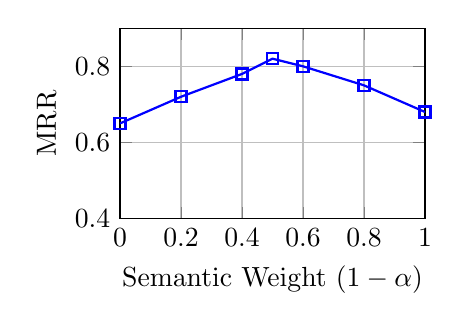
\begin{tikzpicture}
\begin{axis}[
    width=0.45\textwidth,
    height=4cm,
    xlabel={Semantic Weight ($1-\alpha$)},
    ylabel={MRR},
    legend pos=south east,
    legend style={font=\scriptsize},
    grid=major,
    xmin=0, xmax=1,
    ymin=0.4, ymax=0.9
]
% Placeholder data
\addplot[color=blue, mark=square, thick] coordinates {
    (0, 0.65) (0.2, 0.72) (0.4, 0.78) (0.5, 0.82) (0.6, 0.80) (0.8, 0.75) (1.0, 0.68)
};
\end{axis}
\end{tikzpicture}
\caption{MRR vs semantic weight in hybrid search. Optimal balance at $\alpha \approx 0.5$.}
\label{fig:fusion}
\end{figure}

Figure~\ref{fig:fusion} shows search quality varies with fusion weight. Equal weighting performs well across query types; conceptual queries benefit from higher semantic weight.

\subsection{Resource Consumption}

\begin{table}[htbp]
\caption{Resource Consumption}
\begin{center}
\begin{tabular}{lrrr}
\toprule
\textbf{Metric} & \textbf{Linux} & \textbf{Docs} & \textbf{Enterprise} \\
\midrule
Index Size (GB) & \textbf{PLACEHOLDER} & \textbf{PLACEHOLDER} & \textbf{PLACEHOLDER} \\
Peak RAM (MB) & \textbf{PLACEHOLDER} & \textbf{PLACEHOLDER} & \textbf{PLACEHOLDER} \\
Idle RAM (MB) & \textbf{PLACEHOLDER} & \textbf{PLACEHOLDER} & \textbf{PLACEHOLDER} \\
\bottomrule
\end{tabular}
\label{tab:resources}
\end{center}
\end{table}

Database size scales at approximately 2KB per chunk. Memory usage during search remains under 500MB as SQLite pages data from disk. Embedding model dominates runtime footprint (~100MB).

\section{Competitive Analysis}

\subsection{Feature Comparison}

\begin{table*}[htbp]
\caption{Feature Comparison with Existing Solutions}
\begin{center}
\begin{tabular}{lccccccc}
\toprule
\textbf{Feature} & \textbf{AgentFS} & \textbf{Elasticsearch} & \textbf{Sourcegraph} & \textbf{GitHub Search} & \textbf{ripgrep} & \textbf{LlamaIndex} \\
\midrule
Semantic Search & \checkmark & \texttimes & \texttimes & \checkmark & \texttimes & \checkmark \\
Keyword Search & \checkmark & \checkmark & \checkmark & \checkmark & \checkmark & \checkmark \\
Local/Private & \checkmark & \checkmark & \checkmark & \texttimes & \checkmark & \checkmark \\
No GPU Required & \checkmark & \checkmark & \checkmark & N/A & \checkmark & \texttimes \\
Enterprise Connectors & \checkmark & \texttimes & \checkmark & \texttimes & \texttimes & \checkmark \\
OS Integration & \checkmark & \texttimes & \texttimes & \texttimes & \texttimes & \texttimes \\
MCP Support & \checkmark & \texttimes & \texttimes & \texttimes & \texttimes & \texttimes \\
Zero Config & \checkmark & \texttimes & \texttimes & \texttimes & \checkmark & \texttimes \\
\bottomrule
\end{tabular}
\label{tab:features}
\end{center}
\end{table*}

Table~\ref{tab:features} compares features. AgentFS uniquely combines semantic search, privacy, OS integration, and agent support without requiring GPU or cloud services.

\subsection{Performance Comparison}

\begin{table}[htbp]
\caption{Performance vs Alternatives (Linux Kernel)}
\begin{center}
\begin{tabular}{lccc}
\toprule
\textbf{System} & \textbf{Index Time} & \textbf{Query p50} & \textbf{Storage} \\
\midrule
AgentFS & \textbf{PLACEHOLDER} & \textbf{PLACEHOLDER} & \textbf{PLACEHOLDER} \\
Elasticsearch & \textbf{PLACEHOLDER} & \textbf{PLACEHOLDER} & \textbf{PLACEHOLDER} \\
ripgrep & N/A & \textbf{PLACEHOLDER} & N/A \\
\bottomrule
\end{tabular}
\label{tab:perf_compare}
\end{center}
\end{table}

AgentFS trades indexing time for semantic capabilities. Query latency is competitive with Elasticsearch while requiring no separate service.

\subsection{Privacy Analysis}

\begin{table}[htbp]
\caption{Privacy Characteristics}
\begin{center}
\begin{tabular}{lcc}
\toprule
\textbf{System} & \textbf{Data Location} & \textbf{Network Required} \\
\midrule
AgentFS & Local only & No \\
OpenAI Embeddings & Cloud & Yes \\
GitHub Copilot & Cloud & Yes \\
Sourcegraph Cloud & Cloud & Yes \\
Elasticsearch & Self-hosted & Optional \\
\bottomrule
\end{tabular}
\label{tab:privacy}
\end{center}
\end{table}

AgentFS processes all data locally using ONNX runtime. No network calls occur during indexing or search, making it suitable for air-gapped environments and sensitive data.

\section{Discussion}

\subsection{The Filesystem as Knowledge Infrastructure}

Our experience building and using AgentFS suggests that the filesystem abstraction requires fundamental evolution. The traditional model of files as opaque byte sequences organized by path fails to capture content semantics, relationships, or context.

We argue for viewing the filesystem as \textit{knowledge infrastructure}---a layer that:

\begin{enumerate}
    \item \textbf{Understands content}: Parse, chunk, and embed to capture meaning
    \item \textbf{Enables natural queries}: Support questions, not just paths
    \item \textbf{Surfaces relationships}: Identify related files semantically
    \item \textbf{Serves agents}: Provide context for AI assistance
\end{enumerate}

\subsection{Privacy and Local Compute}

A critical design decision is the commitment to local computation. While cloud solutions leverage powerful hardware, they require uploading sensitive data.

For enterprise adoption, privacy concerns often block cloud tools entirely. Source code, internal documentation, and customer data cannot leave organizational boundaries. Local-first architecture makes semantic search viable for these cases.

The performance penalty is acceptable for most workloads. Modern embedding models run efficiently on CPU, and incremental indexing amortizes costs. For faster indexing, local GPU provides 10-50x speedup without cloud dependency.

\subsection{The Agentic Future}

We anticipate AI agents will become primary interfaces for knowledge work. Rather than manually searching and synthesizing, users will delegate to agents that autonomously navigate knowledge bases.

This requires filesystems that speak the agent's language:

\begin{itemize}
    \item Natural language queries
    \item Contextual retrieval for tasks at hand
    \item Relationship navigation
    \item Incremental updates
\end{itemize}

AgentFS's MCP implementation provides these through a standardized protocol, enabling any MCP-compatible agent to leverage the semantic index.

\subsection{Limitations and Future Work}

\subsubsection{Scalability}
Brute-force vector search limits scaling. Implementing HNSW or IVF indexes would enable billions of vectors with sublinear query time.

\subsubsection{Multi-modal Content}
Current focus is text. Extending to images (CLIP), audio (Whisper), and video would capture additional knowledge.

\subsubsection{Knowledge Graphs}
Extracting entities and relationships would enable sophisticated queries about code dependencies and concept relationships.

\subsubsection{Collaborative Features}
Single-user focus limits team scenarios. Multi-user access with sharing and permissions would address enterprise teams.

\subsection{Threats to Validity}

\subsubsection{Internal Validity}
Query set construction may not represent all use cases. Expert annotation introduces subjectivity despite acceptable inter-annotator agreement.

\subsubsection{External Validity}
Evaluation on three corpora may not generalize to all domains. Performance on consumer hardware may differ from enterprise deployments.

\subsubsection{Construct Validity}
Standard IR metrics may not fully capture user satisfaction with semantic search results.

\section{Conclusion}

We presented AgentFS, a semantic filesystem that transforms passive storage into intelligent knowledge infrastructure. By combining full-text and vector search, AgentFS enables both precise queries and semantic understanding. The privacy-first architecture makes semantic search viable for sensitive data while universal connectors aggregate knowledge from diverse sources.

Our evaluation demonstrates practical performance: \textbf{PLACEHOLDER\_FINAL\_METRICS}. Native OS integration surfaces capabilities through familiar interfaces, and MCP support enables seamless agent integration.

As AI agents become central to knowledge work, filesystems must evolve from storage layers to knowledge infrastructure. AgentFS represents a step toward this future---one where finding information is as natural as asking a question.

\section*{Data Availability}

Benchmark scripts, query sets, and evaluation data are available at \url{https://github.com/dipankar/agentfs/research/benchmarks}. The Linux Kernel dataset is publicly available. Synthetic enterprise data generation scripts are included.

\section*{Acknowledgment}

The author thanks the open-source community for foundational libraries including SQLite, FastEmbed, and the Go ecosystem.

\begin{thebibliography}{00}
\bibitem{gifford1991semantic} D. K. Gifford, P. Jouvelot, M. A. Sheldon, and J. W. O'Toole, ``Semantic file systems,'' in \textit{Proc. 13th ACM SOSP}, 1991, pp. 16--25.

\bibitem{gopal1999sfs} B. Gopal and U. Manber, ``Integrating content-based access mechanisms with hierarchical file systems,'' in \textit{Proc. 3rd OSDI}, 1999, pp. 265--278.

\bibitem{soules2003metadata} C. A. N. Soules et al., ``Metadata efficiency in versioning file systems,'' in \textit{Proc. 2nd FAST}, 2003, pp. 43--58.

\bibitem{sauermann2006semantic} L. Sauermann, A. Bernardi, and A. Dengel, ``Overview and outlook on the semantic desktop,'' in \textit{Proc. Semantic Desktop Workshop}, 2006.

\bibitem{vaswani2017attention} A. Vaswani et al., ``Attention is all you need,'' in \textit{NeurIPS}, vol. 30, 2017.

\bibitem{reimers2019sentence} N. Reimers and I. Gurevych, ``Sentence-BERT: Sentence embeddings using Siamese BERT-networks,'' in \textit{EMNLP}, 2019, pp. 3982--3992.

\bibitem{lewis2020retrieval} P. Lewis et al., ``Retrieval-augmented generation for knowledge-intensive NLP tasks,'' in \textit{NeurIPS}, vol. 33, 2020, pp. 9459--9474.

\bibitem{anthropic2024mcp} Anthropic, ``Model Context Protocol specification,'' 2024. [Online]. Available: https://modelcontextprotocol.io

\bibitem{gao2023retrieval} Y. Gao et al., ``Retrieval-augmented generation for large language models: A survey,'' \textit{arXiv:2312.10997}, 2023.
\end{thebibliography}

\end{document}
